\documentclass[11pt]{article}
\usepackage[textwidth=18.0cm, textheight=23.0cm, top=2.0cm]{geometry}
\usepackage{pst-all}
\usepackage{amssymb}
\usepackage{tikz}
\usepackage{underscore}\begin{document}
\pagestyle{empty}


ClassName: \underline{\textbf{Class_03.2bp-14}}
\par
BinSize: \underline{\textbf{40 × 40}}
\par
ReduceSize: \underline{\textbf{40 × 40}}
\par
TypeNum: \underline{\textbf{38}}
\par
Num: \underline{\textbf{40}}
\par
OutS: \underline{\textbf{19200}}
\par
InS: \underline{\textbf{15102}}
\par
Rate: \underline{\textbf{0.787}}
\par
UB: \underline{\textbf{12}}
\par
LB0: \underline{\textbf{12}}
\par
LB: \underline{\textbf{12}}
\par
LBWithCut: \underline{\textbf{12}}
\par
NodeCut: \underline{\textbf{0}}
\par
ExtendedNodeCnt: \underline{\textbf{1}}
\par
GenNodeCnt: \underline{\textbf{1}}
\par
PrimalNode: \underline{\textbf{0}}
\par
ColumnCount: \underline{\textbf{12}}
\par
TotalCutCount: \underline{\textbf{0}}
\par
RootCutCount: \underline{\textbf{0}}
\par
LPSolverCnt: \underline{\textbf{1}}
\par
PricingSolverCnt: \underline{\textbf{0}}
\par
BranchAndBoundNum: \underline{\textbf{1}}
\par
isOpt: \underline{\textbf{true}}
\par
TimeOnPrimal: \underline{\textbf{0.000 s}}
\par
TimeOnPricing: \underline{\textbf{0.000 s}}
\par
TimeOnRmp: \underline{\textbf{0.078 s}}
\par
TotalTime: \underline{\textbf{0.141 s}}
\par
\newpage


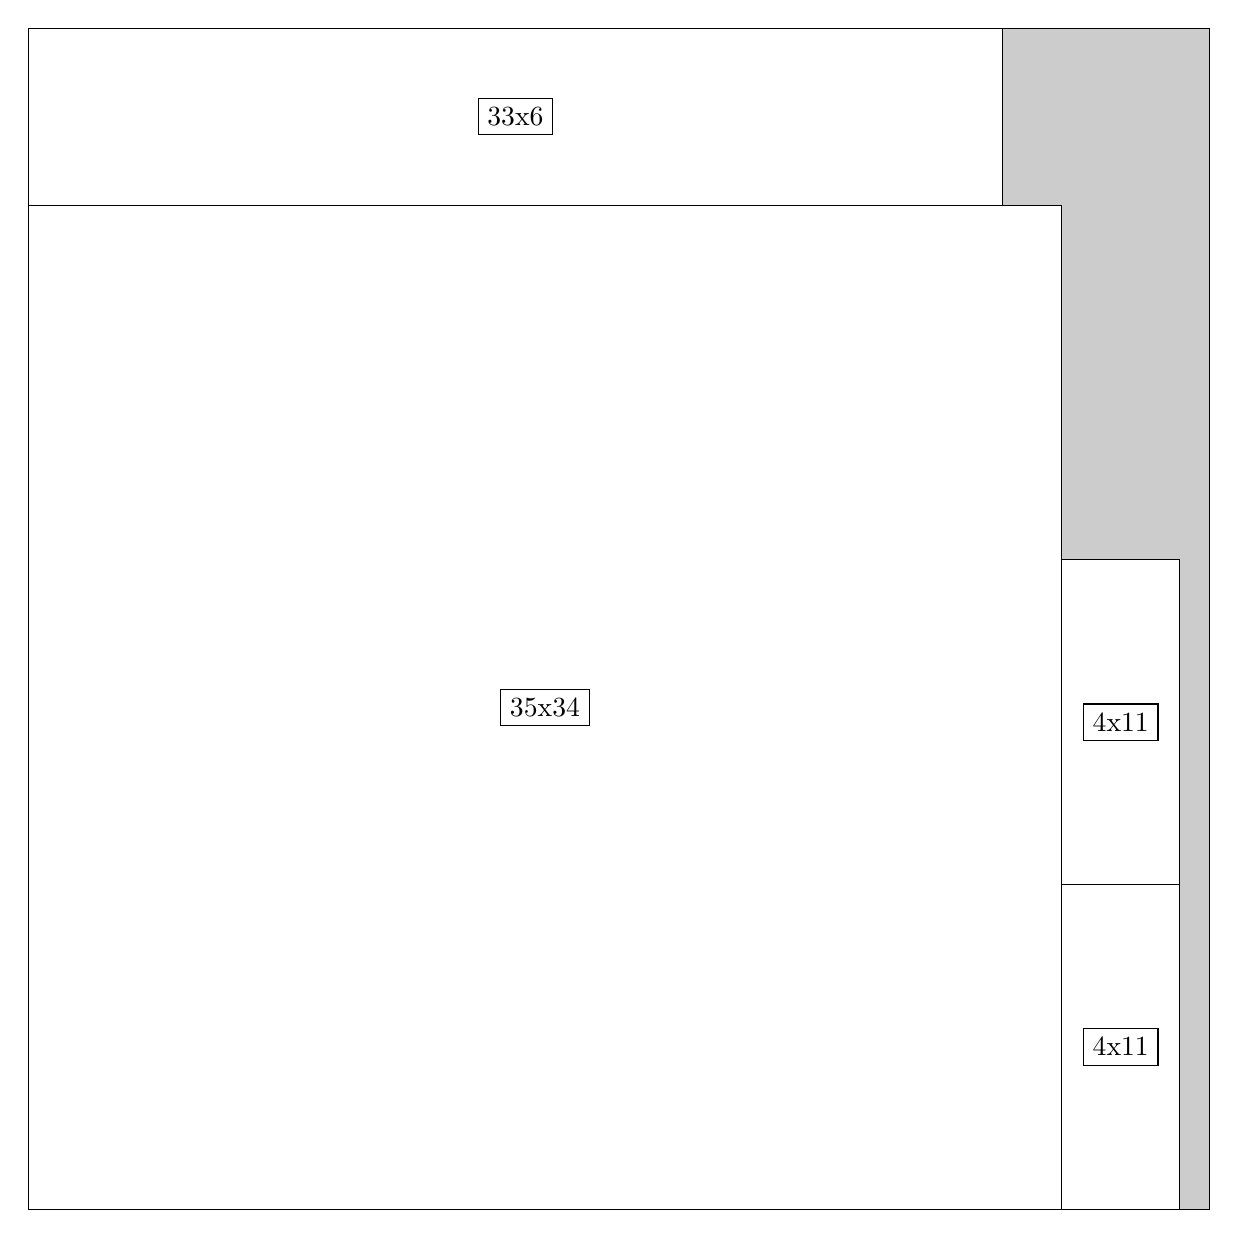
\begin{tikzpicture}[shorten >=1pt,scale=1.0,every node/.style={scale=1.0},->]
\tikzstyle{vertex}=[circle,fill=black!25,minimum size=14pt,inner sep=0pt]
\filldraw[fill=gray!40!white, draw=black] (0,0) rectangle (15.0,15.0);
\foreach \name/\x/\y/\w/\h in {35x34/0.0/0.0/13.125/12.75,33x6/0.0/12.75/12.375/2.25,4x11/13.125/0.0/1.5/4.125,4x11/13.125/4.125/1.5/4.125}
\filldraw[fill=white!40!white, draw=black] (\x,\y) rectangle node[draw] (\name) {\name} ++(\w,\h);
\end{tikzpicture}


w =35 , h =34 , x =0 , y =0 , v =1190
\par
w =33 , h =6 , x =0 , y =34 , v =198
\par
w =4 , h =11 , x =35 , y =0 , v =44
\par
w =4 , h =11 , x =35 , y =11 , v =44
\par
\newpage


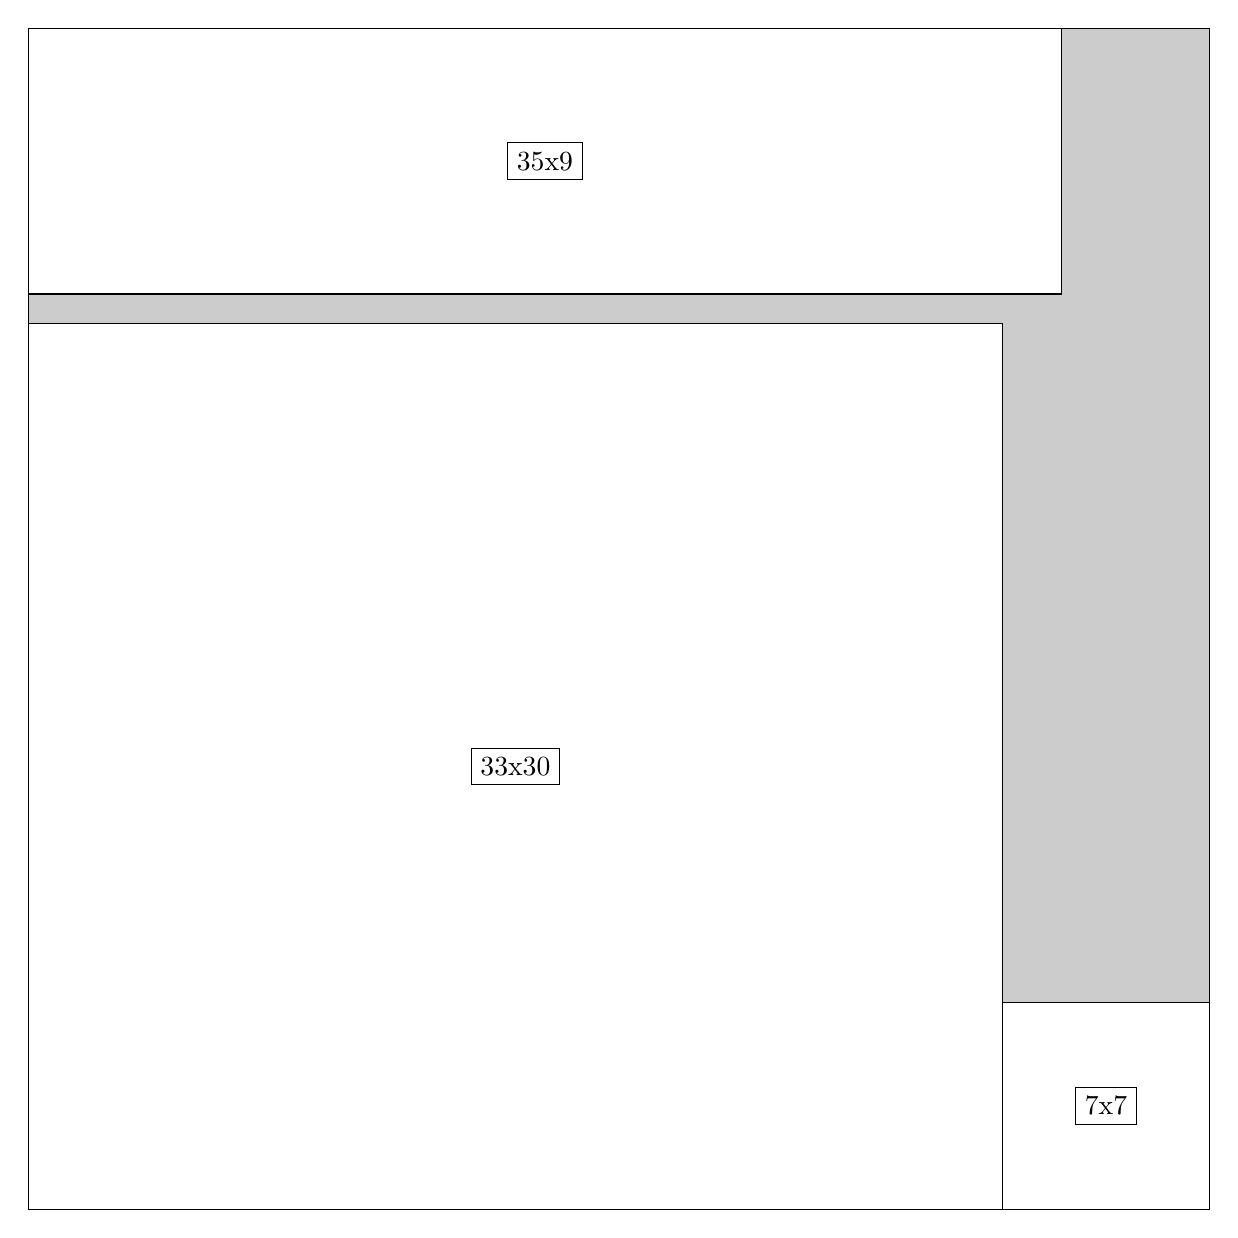
\begin{tikzpicture}[shorten >=1pt,scale=1.0,every node/.style={scale=1.0},->]
\tikzstyle{vertex}=[circle,fill=black!25,minimum size=14pt,inner sep=0pt]
\filldraw[fill=gray!40!white, draw=black] (0,0) rectangle (15.0,15.0);
\foreach \name/\x/\y/\w/\h in {33x30/0.0/0.0/12.375/11.25,35x9/0.0/11.625/13.125/3.375,7x7/12.375/0.0/2.625/2.625}
\filldraw[fill=white!40!white, draw=black] (\x,\y) rectangle node[draw] (\name) {\name} ++(\w,\h);
\end{tikzpicture}


w =33 , h =30 , x =0 , y =0 , v =990
\par
w =35 , h =9 , x =0 , y =31 , v =315
\par
w =7 , h =7 , x =33 , y =0 , v =49
\par
\newpage


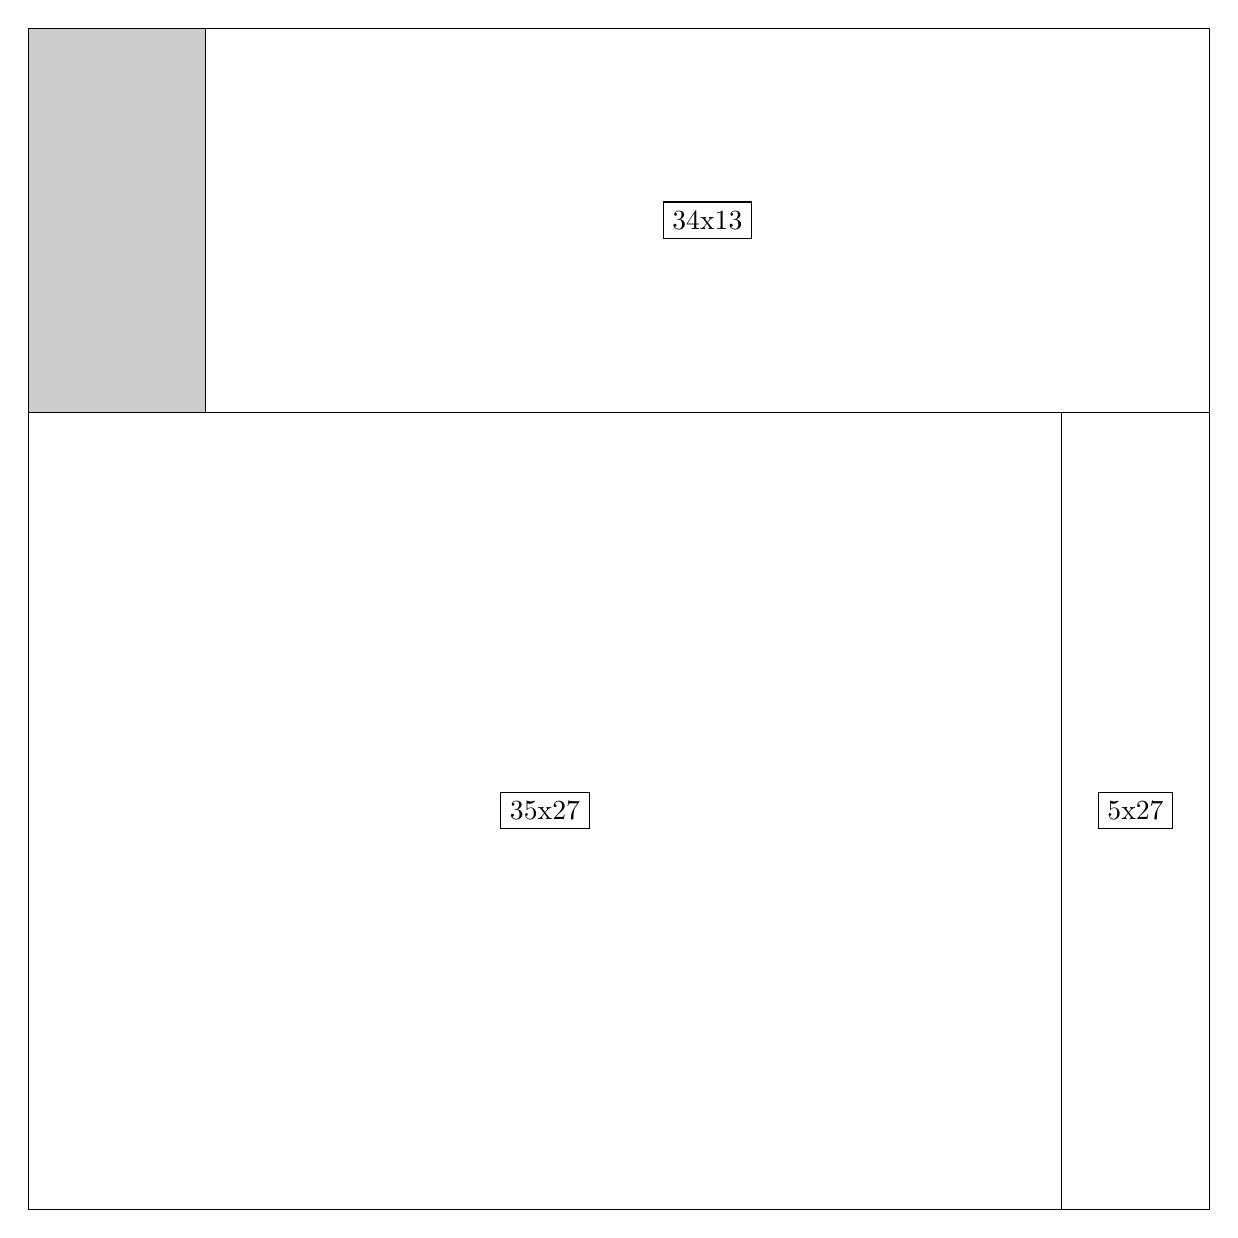
\begin{tikzpicture}[shorten >=1pt,scale=1.0,every node/.style={scale=1.0},->]
\tikzstyle{vertex}=[circle,fill=black!25,minimum size=14pt,inner sep=0pt]
\filldraw[fill=gray!40!white, draw=black] (0,0) rectangle (15.0,15.0);
\foreach \name/\x/\y/\w/\h in {35x27/0.0/0.0/13.125/10.125,34x13/2.25/10.125/12.75/4.875,5x27/13.125/0.0/1.875/10.125}
\filldraw[fill=white!40!white, draw=black] (\x,\y) rectangle node[draw] (\name) {\name} ++(\w,\h);
\end{tikzpicture}


w =35 , h =27 , x =0 , y =0 , v =945
\par
w =34 , h =13 , x =6 , y =27 , v =442
\par
w =5 , h =27 , x =35 , y =0 , v =135
\par
\newpage


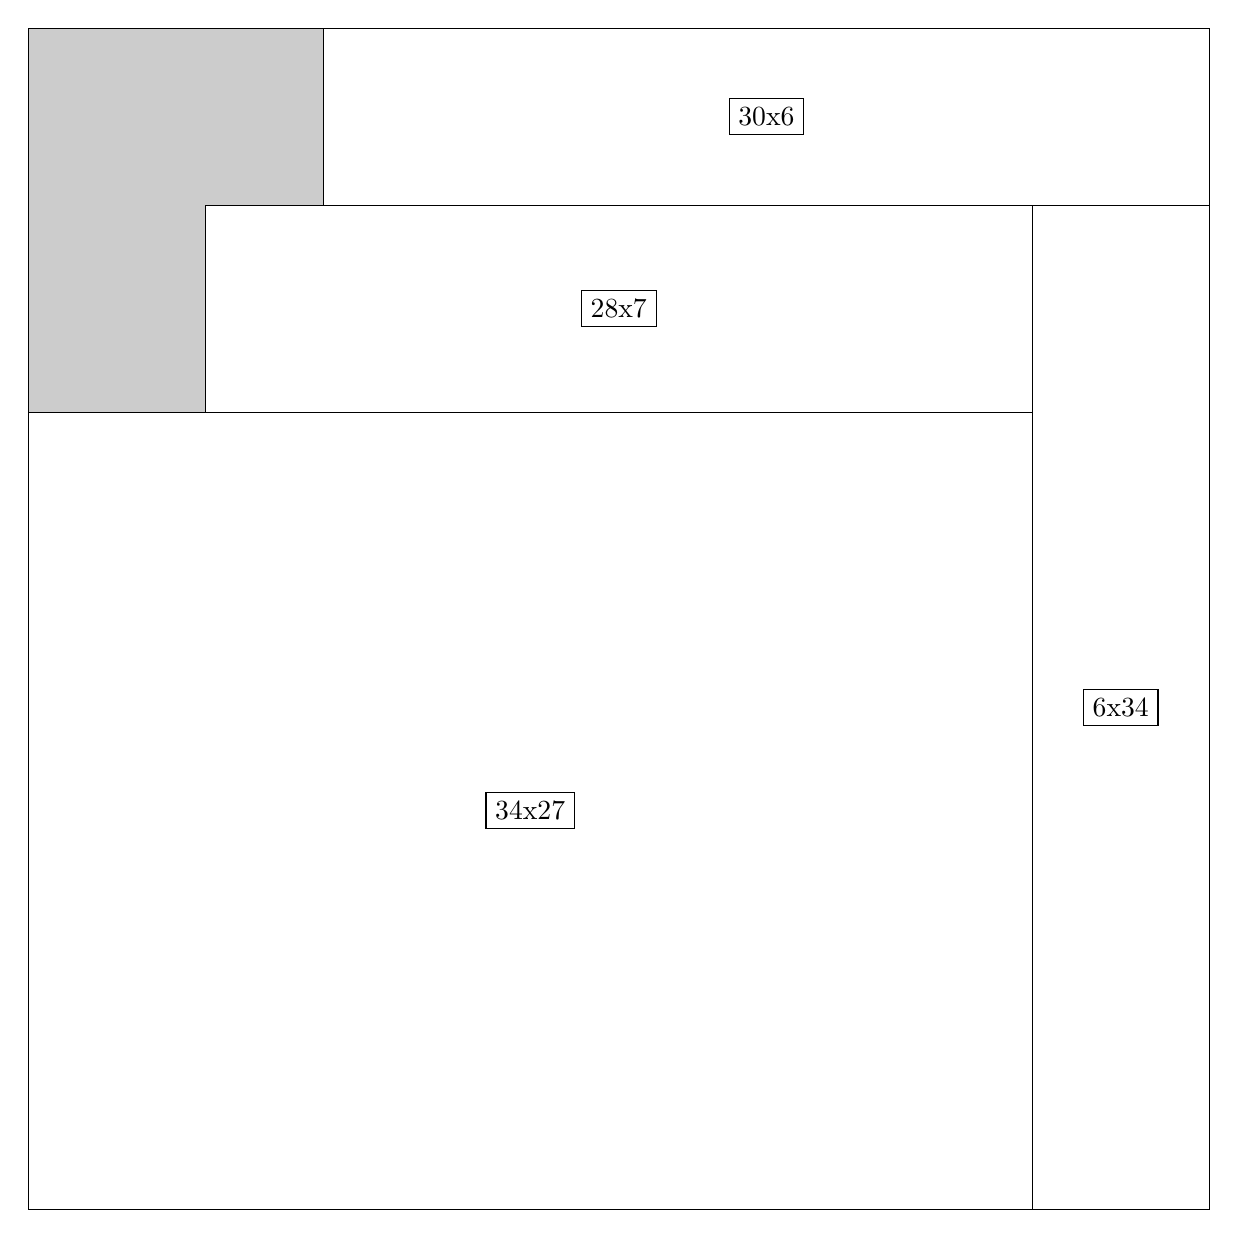
\begin{tikzpicture}[shorten >=1pt,scale=1.0,every node/.style={scale=1.0},->]
\tikzstyle{vertex}=[circle,fill=black!25,minimum size=14pt,inner sep=0pt]
\filldraw[fill=gray!40!white, draw=black] (0,0) rectangle (15.0,15.0);
\foreach \name/\x/\y/\w/\h in {34x27/0.0/0.0/12.75/10.125,6x34/12.75/0.0/2.25/12.75,28x7/2.25/10.125/10.5/2.625,30x6/3.75/12.75/11.25/2.25}
\filldraw[fill=white!40!white, draw=black] (\x,\y) rectangle node[draw] (\name) {\name} ++(\w,\h);
\end{tikzpicture}


w =34 , h =27 , x =0 , y =0 , v =918
\par
w =6 , h =34 , x =34 , y =0 , v =204
\par
w =28 , h =7 , x =6 , y =27 , v =196
\par
w =30 , h =6 , x =10 , y =34 , v =180
\par
\newpage


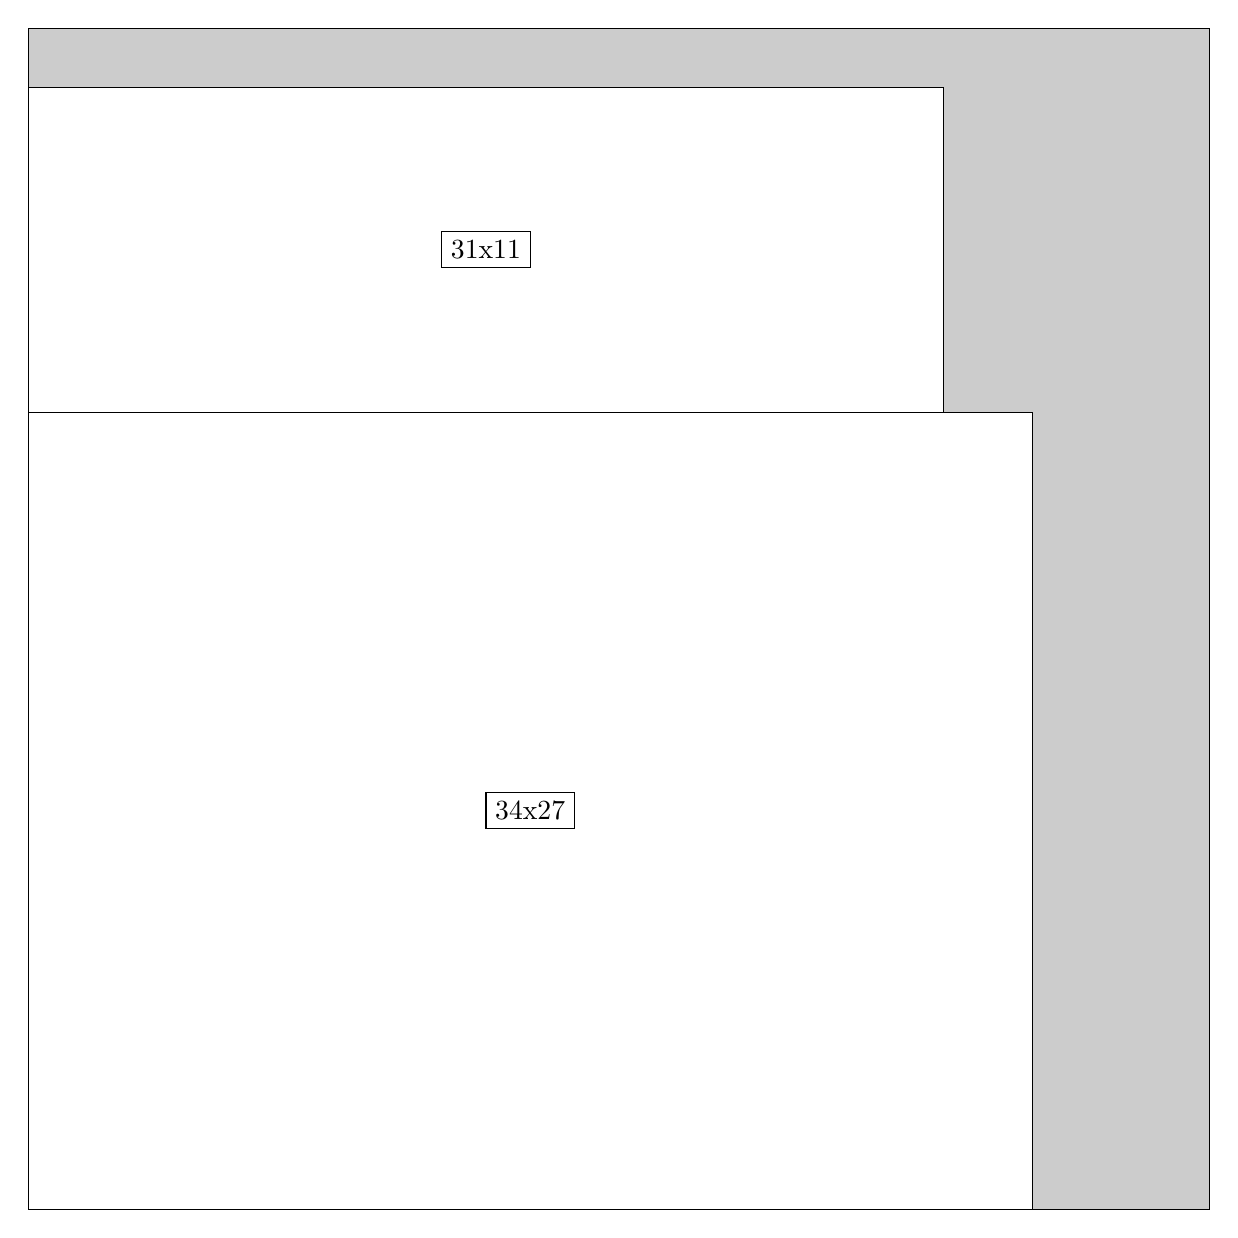
\begin{tikzpicture}[shorten >=1pt,scale=1.0,every node/.style={scale=1.0},->]
\tikzstyle{vertex}=[circle,fill=black!25,minimum size=14pt,inner sep=0pt]
\filldraw[fill=gray!40!white, draw=black] (0,0) rectangle (15.0,15.0);
\foreach \name/\x/\y/\w/\h in {34x27/0.0/0.0/12.75/10.125,31x11/0.0/10.125/11.625/4.125}
\filldraw[fill=white!40!white, draw=black] (\x,\y) rectangle node[draw] (\name) {\name} ++(\w,\h);
\end{tikzpicture}


w =34 , h =27 , x =0 , y =0 , v =918
\par
w =31 , h =11 , x =0 , y =27 , v =341
\par
\newpage


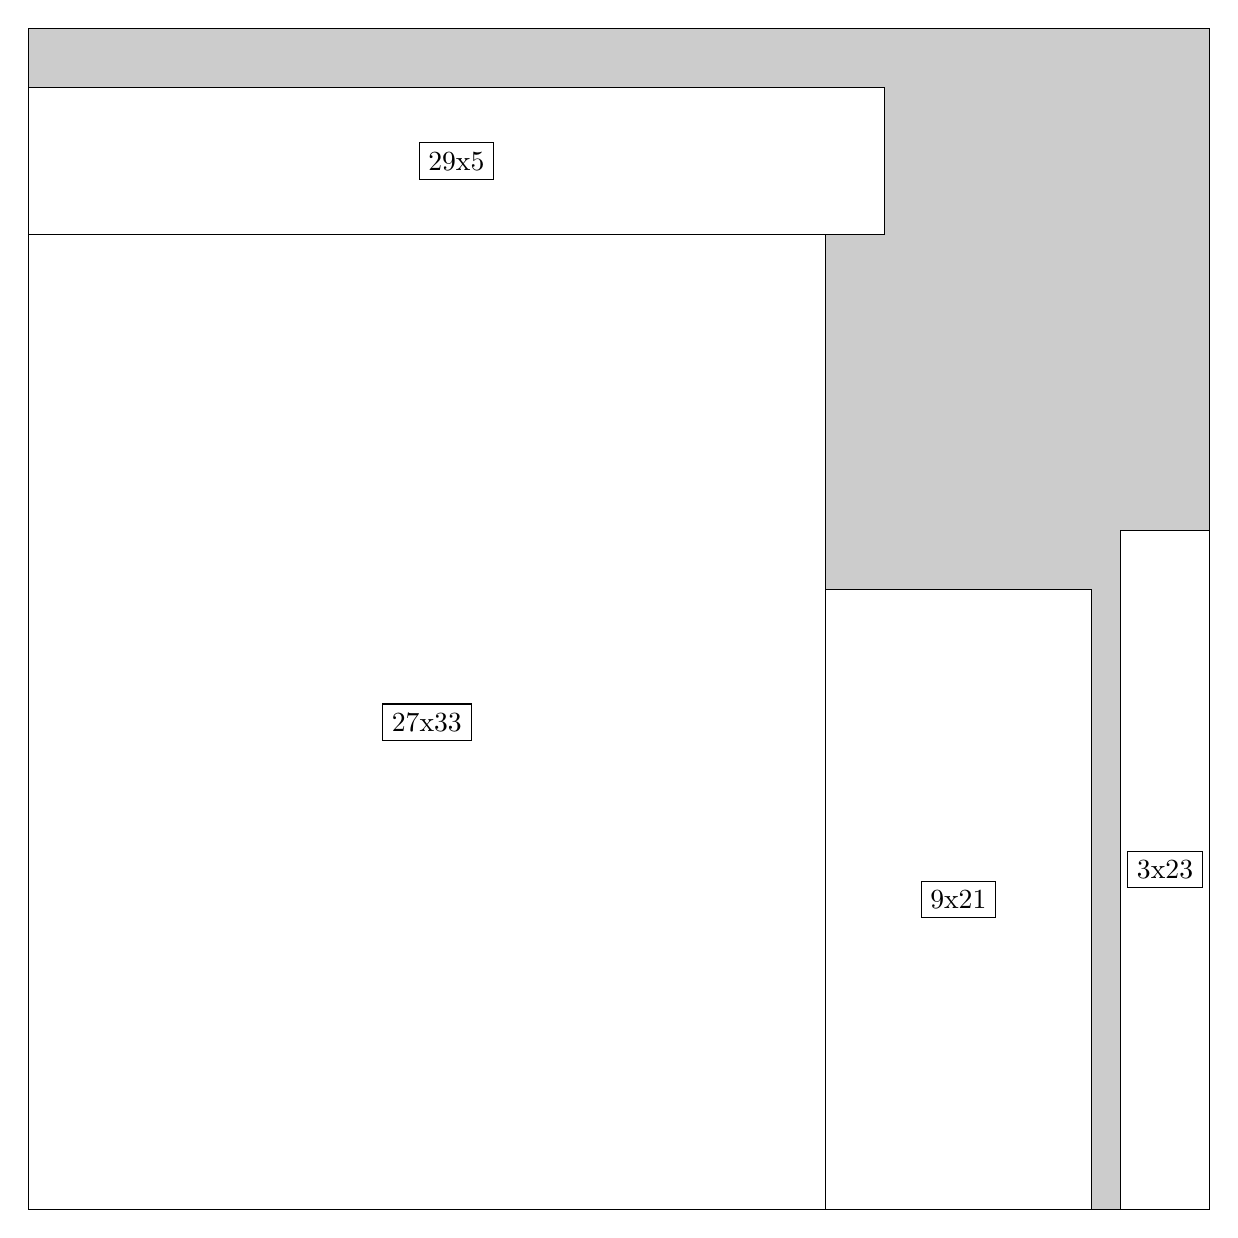
\begin{tikzpicture}[shorten >=1pt,scale=1.0,every node/.style={scale=1.0},->]
\tikzstyle{vertex}=[circle,fill=black!25,minimum size=14pt,inner sep=0pt]
\filldraw[fill=gray!40!white, draw=black] (0,0) rectangle (15.0,15.0);
\foreach \name/\x/\y/\w/\h in {27x33/0.0/0.0/10.125/12.375,9x21/10.125/0.0/3.375/7.875,29x5/0.0/12.375/10.875/1.875,3x23/13.875/0.0/1.125/8.625}
\filldraw[fill=white!40!white, draw=black] (\x,\y) rectangle node[draw] (\name) {\name} ++(\w,\h);
\end{tikzpicture}


w =27 , h =33 , x =0 , y =0 , v =891
\par
w =9 , h =21 , x =27 , y =0 , v =189
\par
w =29 , h =5 , x =0 , y =33 , v =145
\par
w =3 , h =23 , x =37 , y =0 , v =69
\par
\newpage


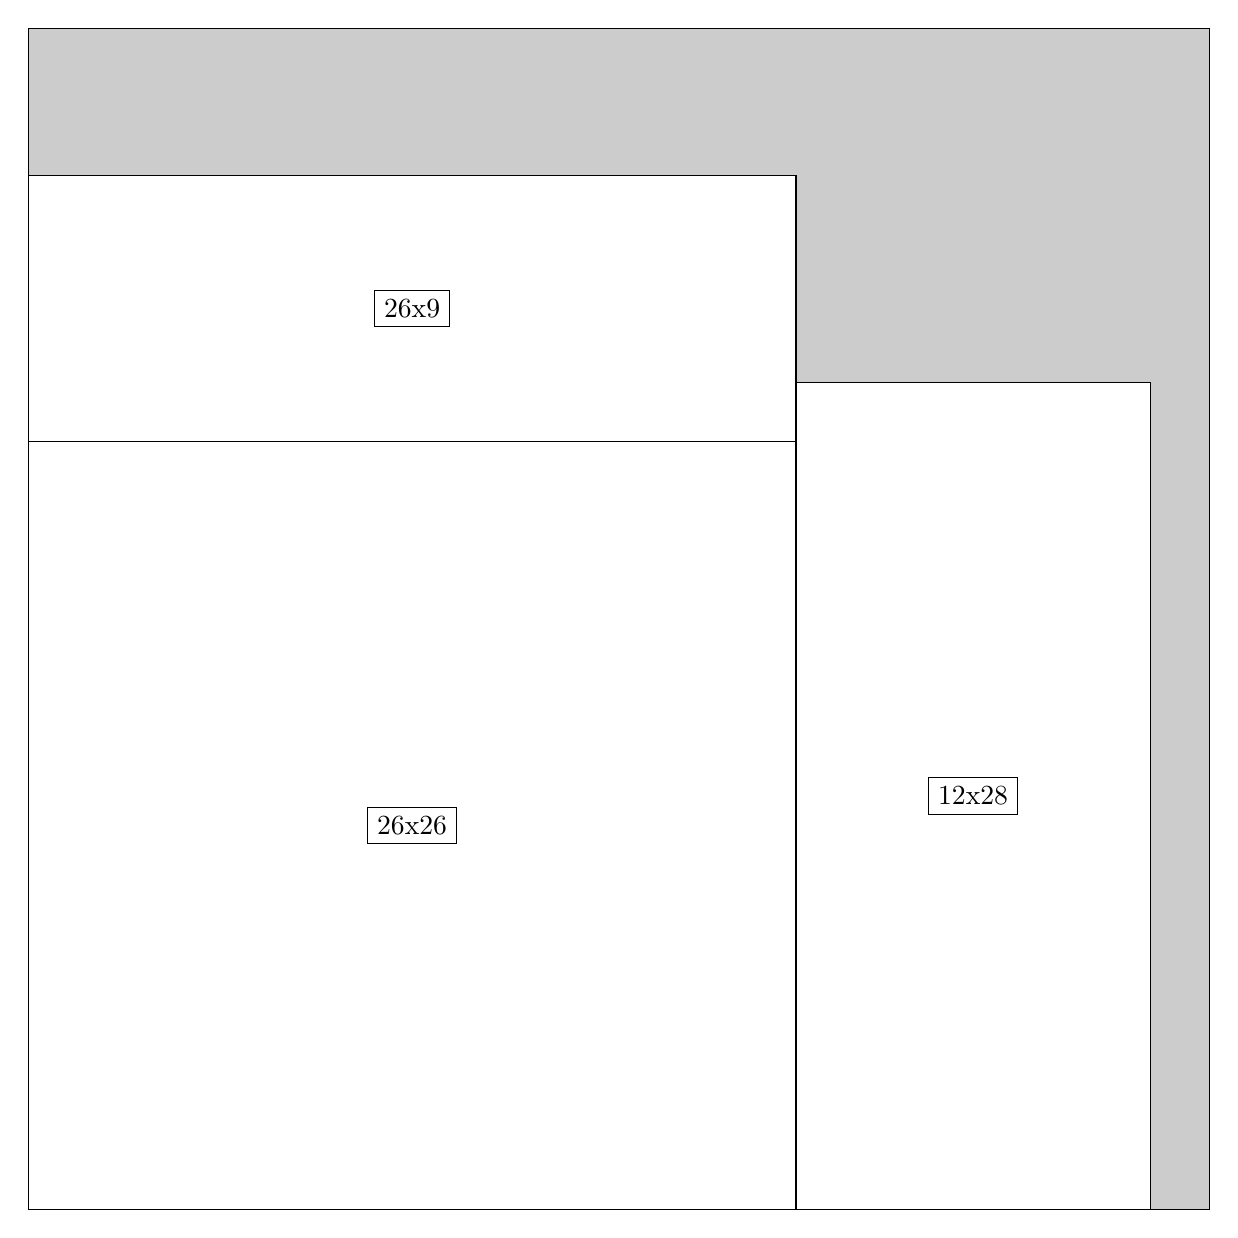
\begin{tikzpicture}[shorten >=1pt,scale=1.0,every node/.style={scale=1.0},->]
\tikzstyle{vertex}=[circle,fill=black!25,minimum size=14pt,inner sep=0pt]
\filldraw[fill=gray!40!white, draw=black] (0,0) rectangle (15.0,15.0);
\foreach \name/\x/\y/\w/\h in {26x26/0.0/0.0/9.75/9.75,12x28/9.75/0.0/4.5/10.5,26x9/0.0/9.75/9.75/3.375}
\filldraw[fill=white!40!white, draw=black] (\x,\y) rectangle node[draw] (\name) {\name} ++(\w,\h);
\end{tikzpicture}


w =26 , h =26 , x =0 , y =0 , v =676
\par
w =12 , h =28 , x =26 , y =0 , v =336
\par
w =26 , h =9 , x =0 , y =26 , v =234
\par
\newpage


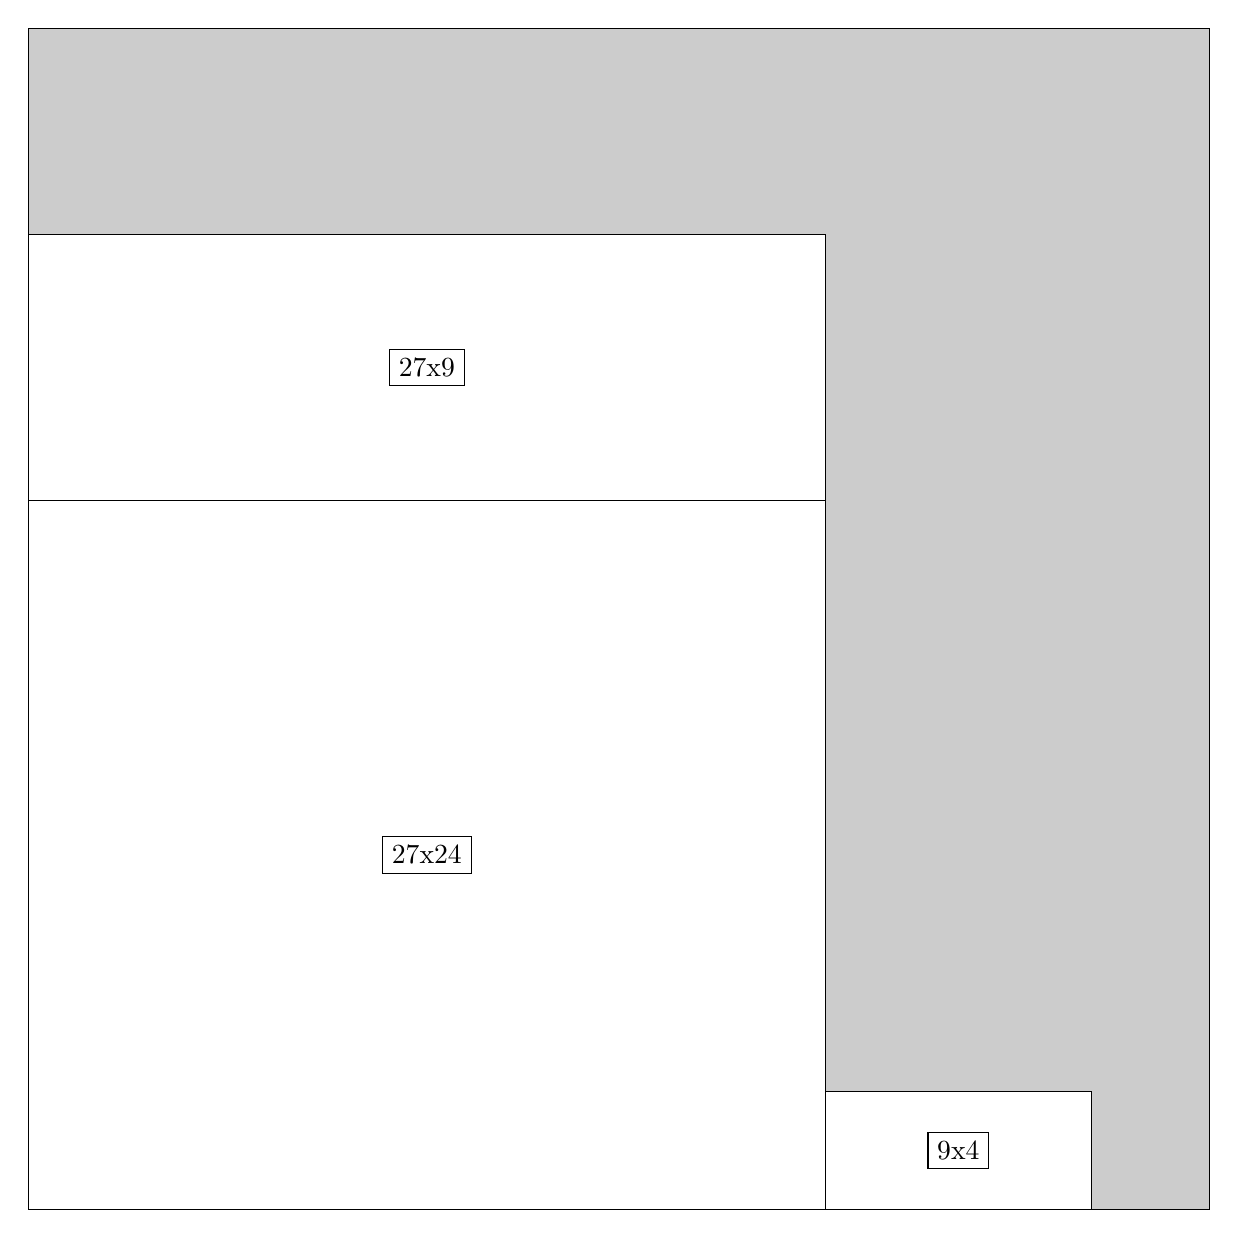
\begin{tikzpicture}[shorten >=1pt,scale=1.0,every node/.style={scale=1.0},->]
\tikzstyle{vertex}=[circle,fill=black!25,minimum size=14pt,inner sep=0pt]
\filldraw[fill=gray!40!white, draw=black] (0,0) rectangle (15.0,15.0);
\foreach \name/\x/\y/\w/\h in {27x24/0.0/0.0/10.125/9.0,27x9/0.0/9.0/10.125/3.375,9x4/10.125/0.0/3.375/1.5}
\filldraw[fill=white!40!white, draw=black] (\x,\y) rectangle node[draw] (\name) {\name} ++(\w,\h);
\end{tikzpicture}


w =27 , h =24 , x =0 , y =0 , v =648
\par
w =27 , h =9 , x =0 , y =24 , v =243
\par
w =9 , h =4 , x =27 , y =0 , v =36
\par
\newpage


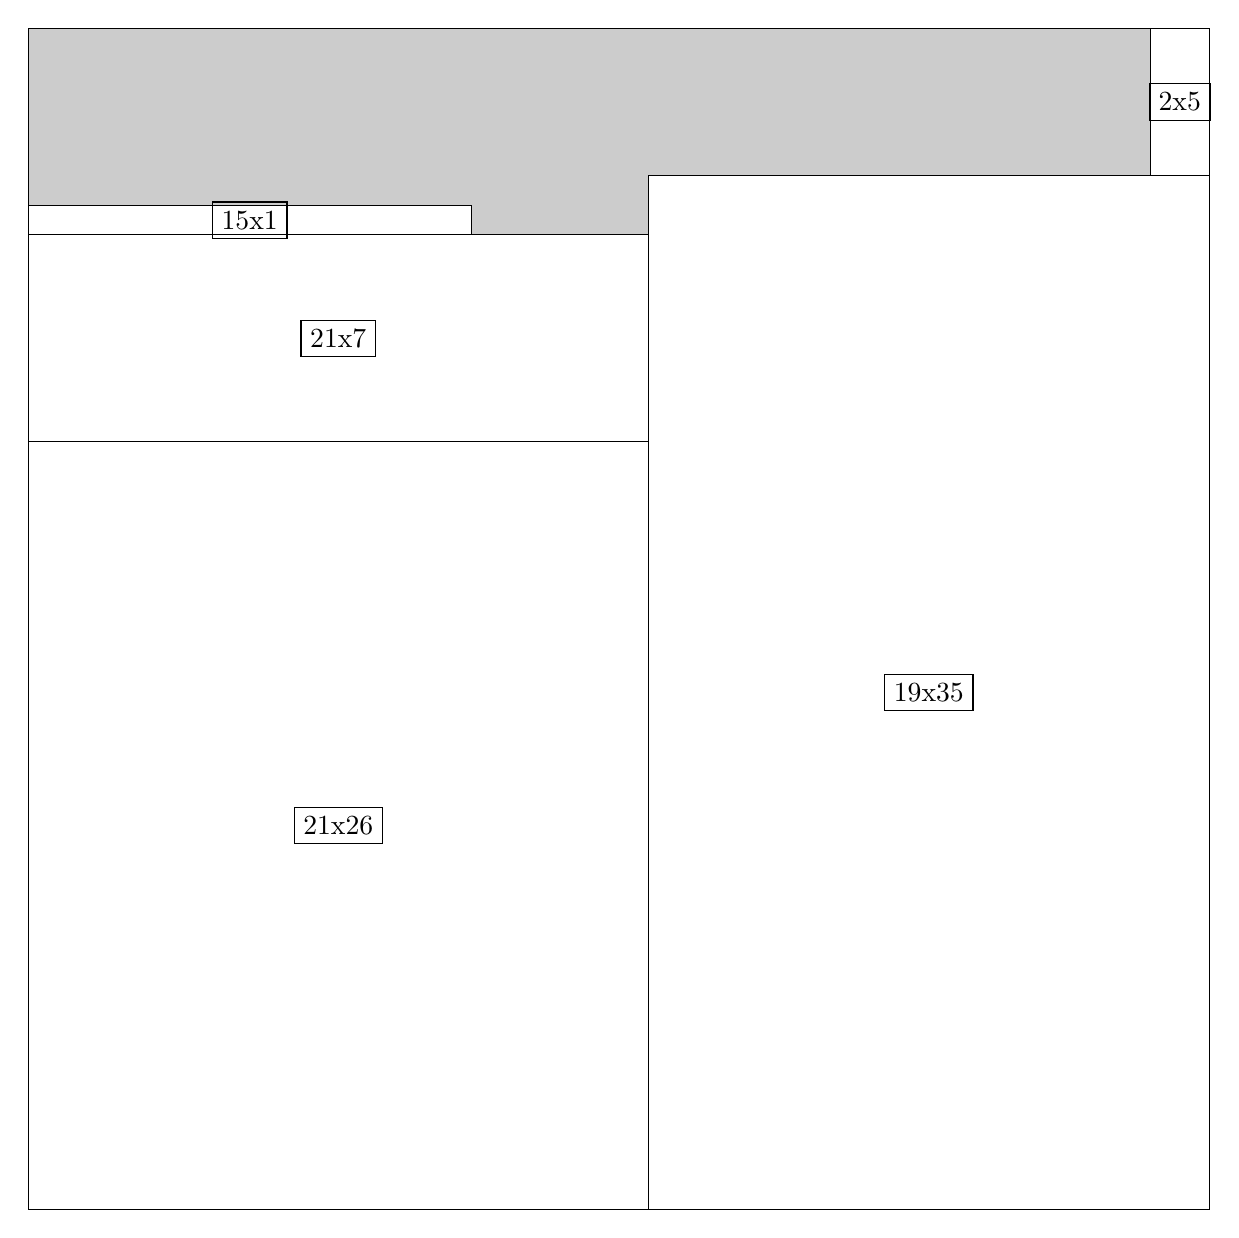
\begin{tikzpicture}[shorten >=1pt,scale=1.0,every node/.style={scale=1.0},->]
\tikzstyle{vertex}=[circle,fill=black!25,minimum size=14pt,inner sep=0pt]
\filldraw[fill=gray!40!white, draw=black] (0,0) rectangle (15.0,15.0);
\foreach \name/\x/\y/\w/\h in {19x35/7.875/0.0/7.125/13.125,21x26/0.0/0.0/7.875/9.75,21x7/0.0/9.75/7.875/2.625,15x1/0.0/12.375/5.625/0.375,2x5/14.25/13.125/0.75/1.875}
\filldraw[fill=white!40!white, draw=black] (\x,\y) rectangle node[draw] (\name) {\name} ++(\w,\h);
\end{tikzpicture}


w =19 , h =35 , x =21 , y =0 , v =665
\par
w =21 , h =26 , x =0 , y =0 , v =546
\par
w =21 , h =7 , x =0 , y =26 , v =147
\par
w =15 , h =1 , x =0 , y =33 , v =15
\par
w =2 , h =5 , x =38 , y =35 , v =10
\par
\newpage


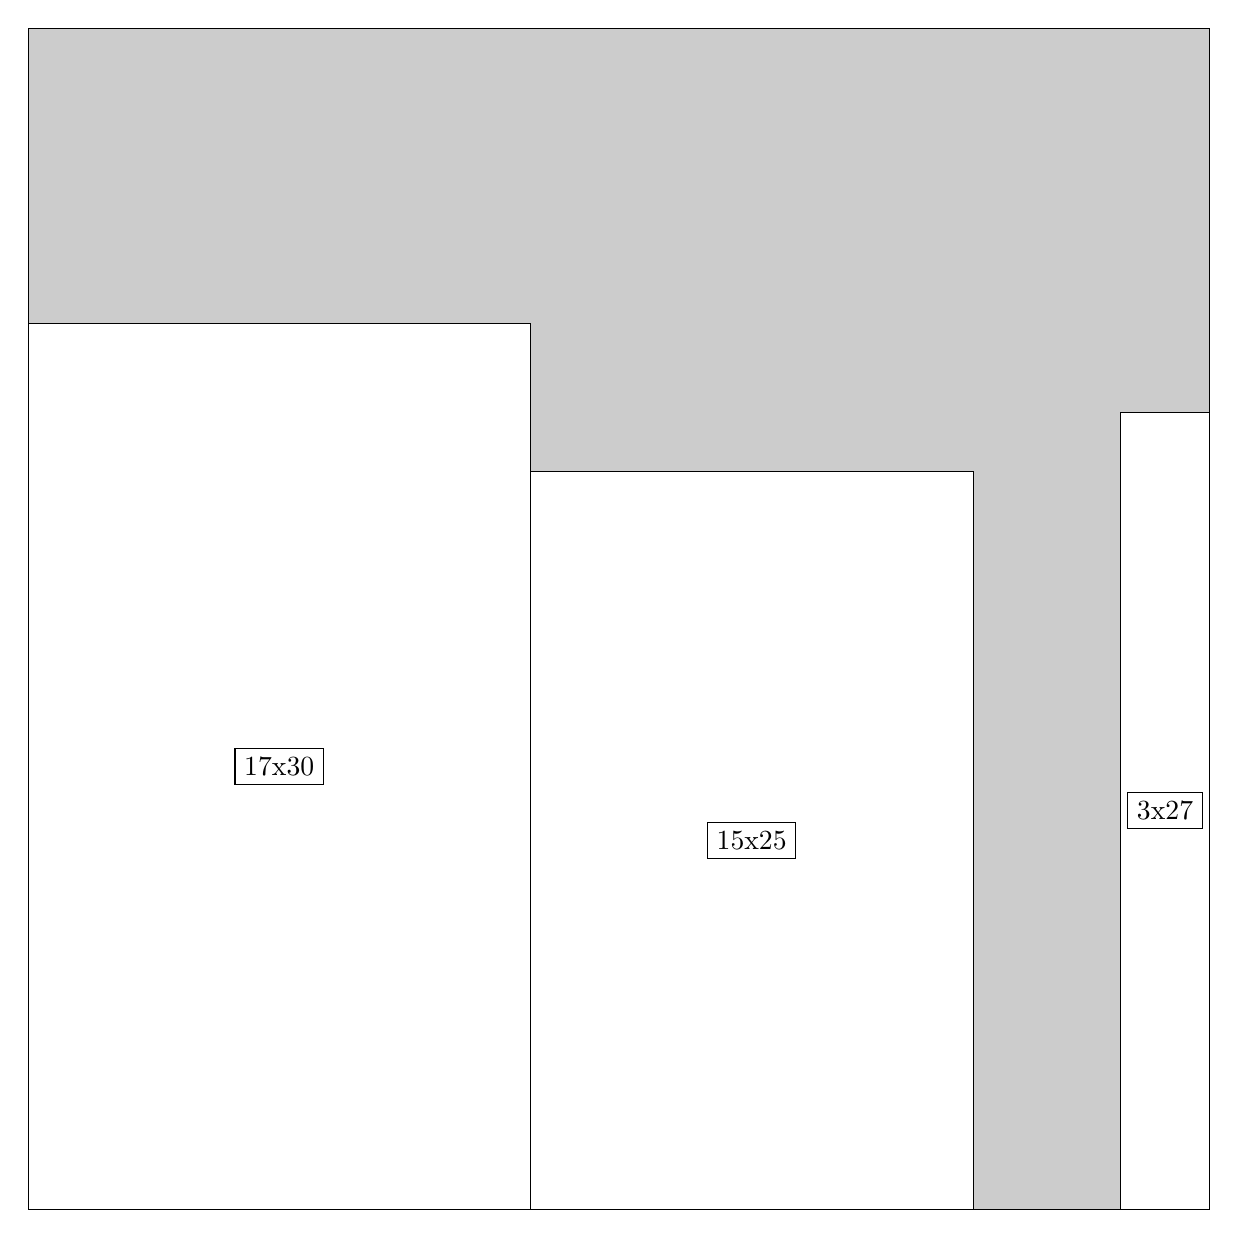
\begin{tikzpicture}[shorten >=1pt,scale=1.0,every node/.style={scale=1.0},->]
\tikzstyle{vertex}=[circle,fill=black!25,minimum size=14pt,inner sep=0pt]
\filldraw[fill=gray!40!white, draw=black] (0,0) rectangle (15.0,15.0);
\foreach \name/\x/\y/\w/\h in {17x30/0.0/0.0/6.375/11.25,15x25/6.375/0.0/5.625/9.375,3x27/13.875/0.0/1.125/10.125}
\filldraw[fill=white!40!white, draw=black] (\x,\y) rectangle node[draw] (\name) {\name} ++(\w,\h);
\end{tikzpicture}


w =17 , h =30 , x =0 , y =0 , v =510
\par
w =15 , h =25 , x =17 , y =0 , v =375
\par
w =3 , h =27 , x =37 , y =0 , v =81
\par
\newpage


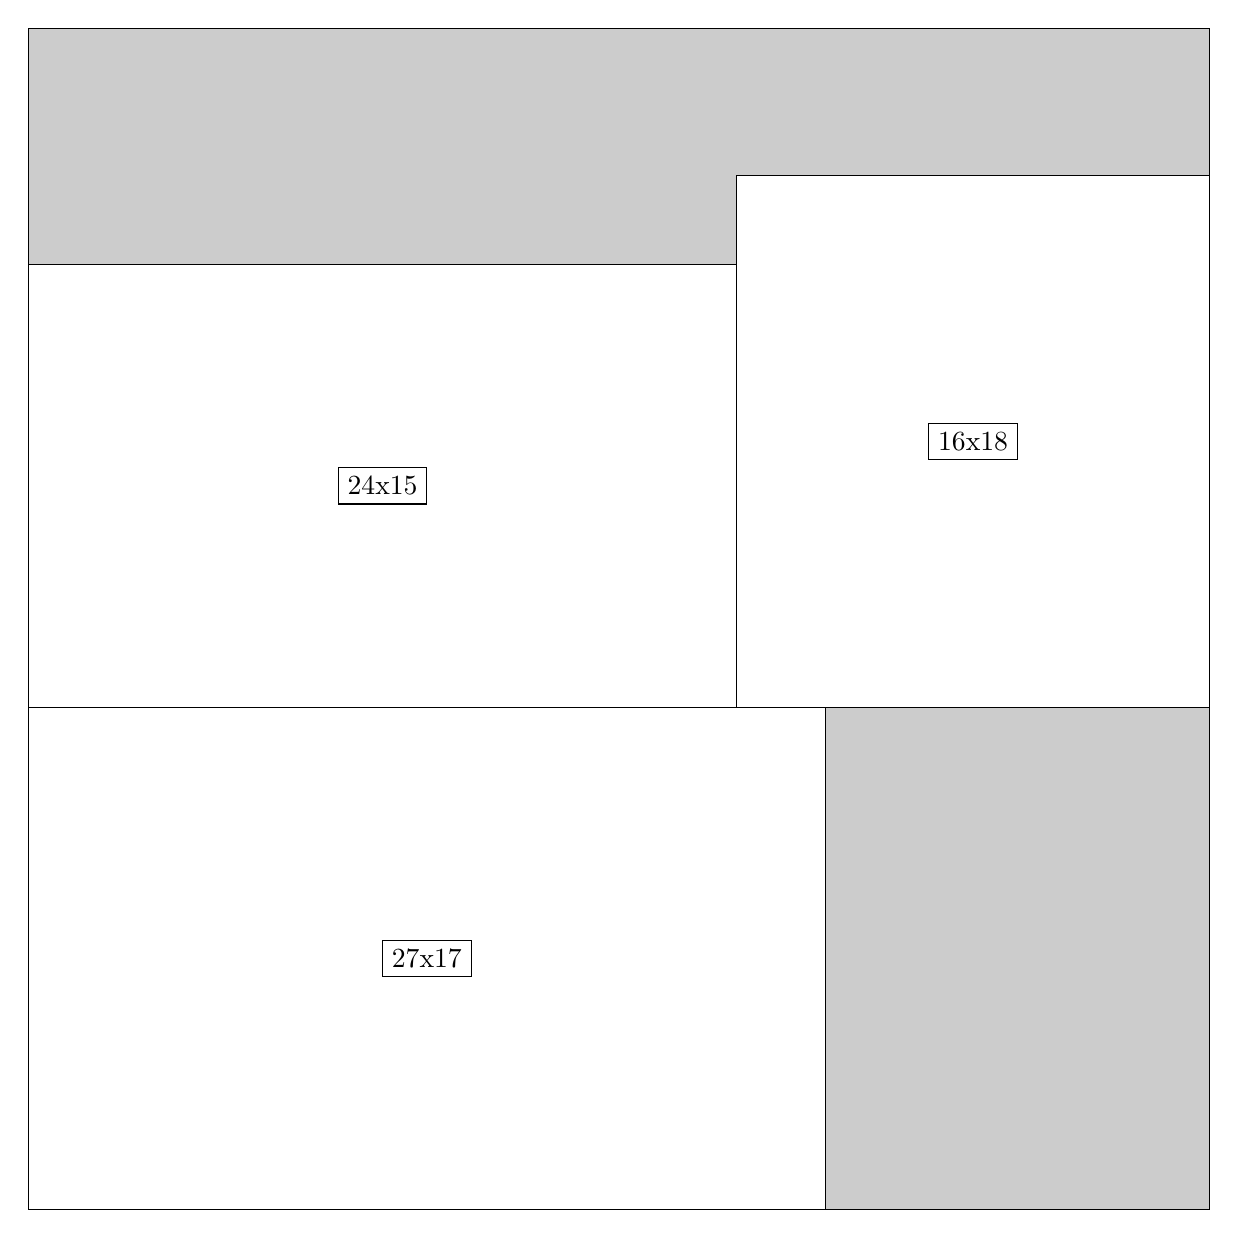
\begin{tikzpicture}[shorten >=1pt,scale=1.0,every node/.style={scale=1.0},->]
\tikzstyle{vertex}=[circle,fill=black!25,minimum size=14pt,inner sep=0pt]
\filldraw[fill=gray!40!white, draw=black] (0,0) rectangle (15.0,15.0);
\foreach \name/\x/\y/\w/\h in {27x17/0.0/0.0/10.125/6.375,24x15/0.0/6.375/9.0/5.625,16x18/9.0/6.375/6.0/6.75}
\filldraw[fill=white!40!white, draw=black] (\x,\y) rectangle node[draw] (\name) {\name} ++(\w,\h);
\end{tikzpicture}


w =27 , h =17 , x =0 , y =0 , v =459
\par
w =24 , h =15 , x =0 , y =17 , v =360
\par
w =16 , h =18 , x =24 , y =17 , v =288
\par
\newpage


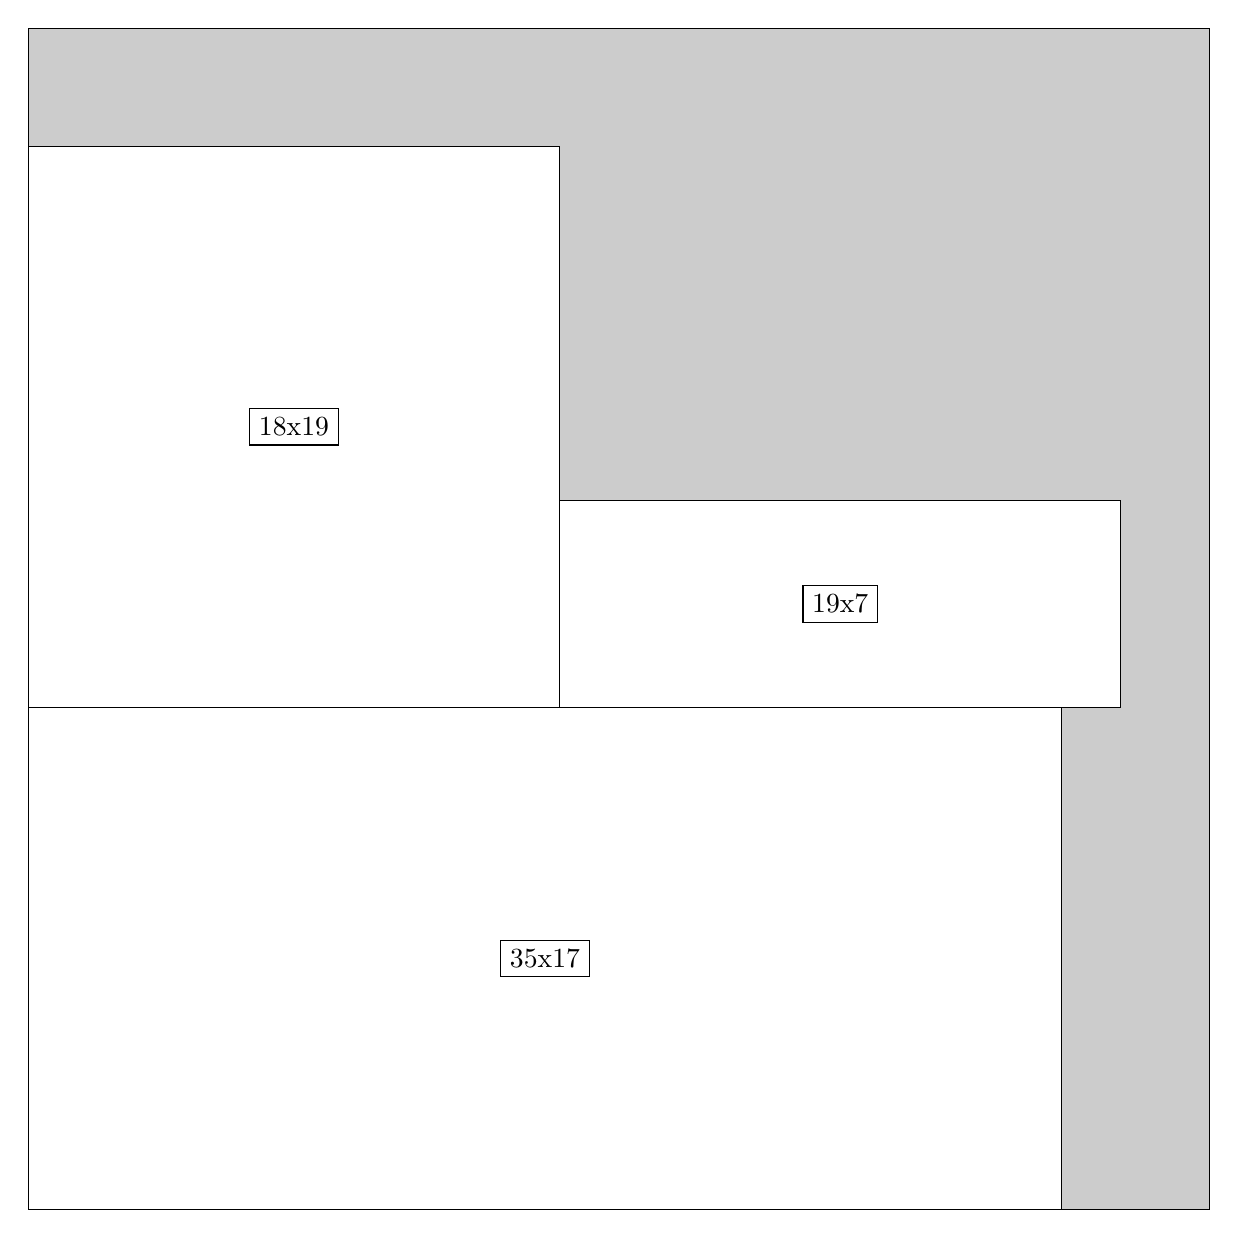
\begin{tikzpicture}[shorten >=1pt,scale=1.0,every node/.style={scale=1.0},->]
\tikzstyle{vertex}=[circle,fill=black!25,minimum size=14pt,inner sep=0pt]
\filldraw[fill=gray!40!white, draw=black] (0,0) rectangle (15.0,15.0);
\foreach \name/\x/\y/\w/\h in {35x17/0.0/0.0/13.125/6.375,18x19/0.0/6.375/6.75/7.125,19x7/6.75/6.375/7.125/2.625}
\filldraw[fill=white!40!white, draw=black] (\x,\y) rectangle node[draw] (\name) {\name} ++(\w,\h);
\end{tikzpicture}


w =35 , h =17 , x =0 , y =0 , v =595
\par
w =18 , h =19 , x =0 , y =17 , v =342
\par
w =19 , h =7 , x =18 , y =17 , v =133
\par
\newpage


\end{document}